\PassOptionsToPackage{unicode=true}{hyperref} % options for packages loaded elsewhere
\PassOptionsToPackage{hyphens}{url}
%
\documentclass[]{article}
\usepackage[margin=0.5in]{geometry}
\usepackage{fancyhdr}
\pagestyle{fancy}
\usepackage{titling}
\usepackage{multicol}
\usepackage{lmodern}
\usepackage{amssymb,amsmath}
\usepackage{ifxetex,ifluatex}
\usepackage{fixltx2e} % provides \textsubscript
\usepackage[T1]{fontenc}
\ifnum 0\ifxetex 1\fi\ifluatex 1\fi=0 % if pdftex
  \usepackage[utf8]{inputenc}
  \usepackage{textcomp} % provides euro and other symbols
\else % if luatex or xelatex
  \usepackage{unicode-math}
  \defaultfontfeatures{Ligatures=TeX,Scale=MatchLowercase}
\fi
% use microtype if available
\IfFileExists{microtype.sty}{%
\usepackage[]{microtype}
\UseMicrotypeSet[protrusion]{basicmath} % disable protrusion for tt fonts
}{}
\IfFileExists{parskip.sty}{%
\usepackage{parskip}
}{% else
\setlength{\parindent}{0pt}
\setlength{\parskip}{6pt plus 2pt minus 1pt}
}
\usepackage{hyperref}
\hypersetup{
            pdfborder={0 0 0},
            breaklinks=true}
\urlstyle{same}  % don't use monospace font for urls
\usepackage{longtable,booktabs}
% Fix footnotes in tables (requires footnote package)
\IfFileExists{footnote.sty}{\usepackage{footnote}\makesavenoteenv{longtable}}{}
\usepackage{graphicx,grffile}
\makeatletter
\def\maxwidth{\ifdim\Gin@nat@width>\linewidth\linewidth\else\Gin@nat@width\fi}
\def\maxheight{\ifdim\Gin@nat@height>\textheight\textheight\else\Gin@nat@height\fi}
\makeatother
% Scale images if necessary, so that they will not overflow the page
% margins by default, and it is still possible to overwrite the defaults
% using explicit options in \includegraphics[width, height, ...]{}
\setkeys{Gin}{width=\maxwidth,height=\maxheight,keepaspectratio}
\setlength{\emergencystretch}{3em}  % prevent overfull lines
\providecommand{\tightlist}{%
  \setlength{\itemsep}{0pt}\setlength{\parskip}{0pt}}
\setcounter{secnumdepth}{0}
% Redefines (sub)paragraphs to behave more like sections
\ifx\paragraph\undefined\else
\let\oldparagraph\paragraph
\renewcommand{\paragraph}[1]{\oldparagraph{#1}\mbox{}}
\fi
\ifx\subparagraph\undefined\else
\let\oldsubparagraph\subparagraph
\renewcommand{\subparagraph}[1]{\oldsubparagraph{#1}\mbox{}}
\fi


\usepackage[table]{xcolor}
\definecolor{lightgray}{gray}{0.9}
\definecolor{midgray}{RGB}{102,102,102}

% alternate rowcolors for all tables
\let\oldtabular\tabular
\let\endoldtabular\endtabular
\renewenvironment{tabular}{\rowcolors{2}{white}{lightgray}\oldtabular}{\endoldtabular}

% alternate rowcolors for all long-tables
\let\oldlongtable\longtable
\let\endoldlongtable\endlongtable
\renewenvironment{longtable}{\rowcolors{2}{white}{lightgray}\oldlongtable} {
\endoldlongtable}

% set default figure placement to htbp
\makeatletter
\def\fps@figure{htbp}
\makeatother


\date{}

\usepackage[sfdefault,light]{merriweather}

%%%%%%%%%%%%  HEADER  %%%%%%%%%%%%%%
\renewcommand{\headrulewidth}{0pt}
\lhead{}
\rhead{}

%%%%%%%%%%%%  FOOTER  %%%%%%%%%%%%%%

\renewcommand{\footrulewidth}{1pt}
\lfoot{Bulock Home Technical Systems}
\cfoot{Revision 1d ~ 2017-12-07}
\rfoot{\thepage}

\begin{document}
%%%%%%%%%%%%  ToC  %%%%%%%%%%%%%%

\pretitle{\begin{center}\fontsize{30bp}{30bp}\selectfont}
\posttitle{\par\end{center}}
\title{\color{midgray}\textbf{Bulock Home Technical Systems}}

\maketitle

\tableofcontents


 %%%%%%%%%%%%  Internet Service Provider  %%%%%%%%%%%%%%

\newpage

\vspace{\baselineskip}\section*{Internet Service Provider}
\addcontentsline{toc}{section}{Internet Service Provider}

\textbf{Service Provider: }
{Wide Open West (WOW!)}

\textbf{Contact: }
{1-866-496-9669}

\textbf{Account Number: }
{14364727}

\textbf{Service: }
{110M down / 10M up}

\textbf{Modem: }
{ARRIS SURFboard SB6183}

\textbf{Modem HFC MAC: }
\texttt{78:96:84:e8:28:ee}

\textbf{Modem Web Interface: }
{\href{https://www.google.com/url?q=http://192.168.100.1\&sa=D\&ust=1544293199830000}{http://192.168.100.1}}


\subsection{\texorpdfstring{{Network}}{Network}}

\textbf{Router: }
{Ubiquiti EdgeRouter X SFP}

\textbf{Router Web Interface: }
{\href{https://www.google.com/url?q=https://router/\&sa=D\&ust=1544293199833000}{https://router/}}

\textbf{Primary Switch: }
{UniFi Switch 24}

\textbf{UniFi Cloud Controller: }
{\href{https://www.google.com/url?q=https://unifi:8443/\&sa=D\&ust=1544293199834000}{https://unifi:8443/}}


%%%%%%%%%%%%  Ethernet Layout %%%%%%%%%%%%%%

\newpage

\vspace{\baselineskip}\section*{Ethernet Layout}
\addcontentsline{toc}{section}{Ethernet Layout}

\begin{multicols}{2}

\subsection{\texorpdfstring{{Patch Panel}}{Patch Panel}}

\begin{enumerate}
\item
  {Office}
\item
  {Living Room}
\item
  {Loft WAP}
\item
  {Loft}
\item
  {Hailey's Room}
\item
  {Master Bedroom}
\item
  {Brett's Room}
\item
  {Basement WAP}
\item
  {Living Room}
\item
  {Unused}
\item
  {Unused}
\item
  {Unused}
\item
  {Unused}
\item
  {Unused}
\item
  {Unused}
\item
  {Unused}
\end{enumerate}

{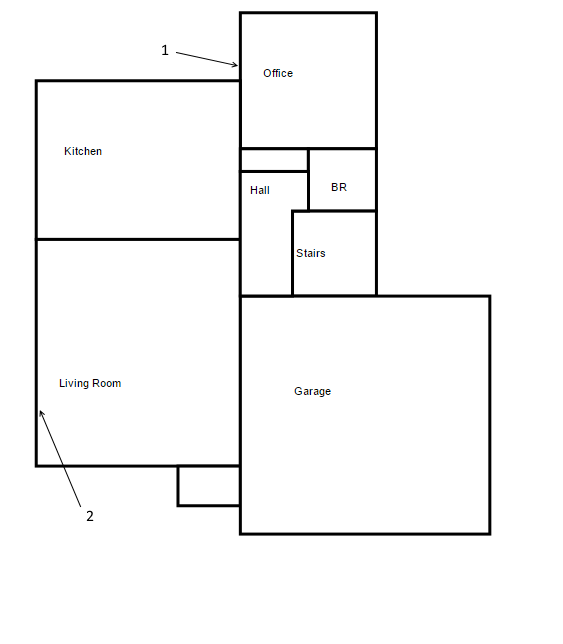
\includegraphics[width=0.45\textwidth]{images/main_floor.png}}
{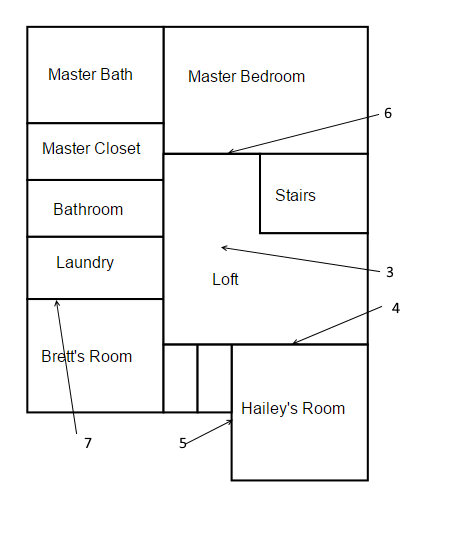
\includegraphics[width=0.45\textwidth]{images/upstairs.png}}

\end{multicols}
%%%%%%%%%%%%  Wireless Network %%%%%%%%%%%%%%

\newpage

\vspace{\baselineskip}\section*{Wireless Network}
\addcontentsline{toc}{section}{Wireless Network}

\textbf{SSID: }
{BulockWireless}

\textbf{Guest SSID: }
{BulockGuestServices}

\subsection{\texorpdfstring{{Controller}}{Controller}}

\textbf{Hardware: }
{Ubiquiti UniFi Cloud Key}

\textbf{Controller MAC: }
\texttt{f0:9f:c2:18:5d:e0}

\textbf{Controller IP: }
{10.0.0.3}

\textbf{Controller Web Interface: }
{\href{https://www.google.com/url?q=https://unifi:8443\&sa=D\&ust=1544293199842000}{https://unifi:8443}}

\textbf{Controller Username: }
{admin}

\subsection{\texorpdfstring{{Access Points}}{Access Points}}

\paragraph{\texorpdfstring{{Loft}}{Loft}}

\textbf{Hardware: }
{UniFi AP-AC-Lite}

\textbf{AP MAC: }
\texttt{44:d9:e7:f6:c8:34}

\textbf{AP IP: }
{10.0.10.2}

\paragraph{\texorpdfstring{{Basement}}{Basement}}

\textbf{Hardware: }
{UniFi AP-AC-Lite}

\textbf{AP MAC: }
\texttt{80:2a:a8:13:15:51}

\textbf{AP IP: }
{10.0.10.0}

%%%%%%%%%%%%  Network Services %%%%%%%%%%%%%%

\newpage

\vspace{\baselineskip}\section*{Network Services}
\addcontentsline{toc}{section}{Network Services}

\subsection{\texorpdfstring{{DNS}}{DNS}}

\textbf{Device: }
{Ubiquiti EdgeRouter X SFP}

\textbf{IP Address: }
{10.0.0.1}

\subsection{\texorpdfstring{{DHCP}}{DHCP}}

\textbf{Device: }
{Ubiquiti EdgeRouter X SFP}

\textbf{IP Address: }
{10.0.0.1}

\subsection{\texorpdfstring{{Reverse Proxy}}{Reverse Proxy}}

\textbf{Device: }
{Raspberry Pi 2 App Server}

\textbf{IP Address: }
{10.0.0.20}

\textbf{Platform: }
{Nginx}

\subsection{\texorpdfstring{{Plex Media Server}}{Plex Media Server}}

\textbf{Device: }
{QNAP TS-453A NAS}

\textbf{IP Address: }
{10.0.0.25}

 %%%%%%%%%%%%  Databases / Data %%%%%%%%%%%%%%

 \newpage

 \vspace{\baselineskip}\section*{Databases / Data}
 \addcontentsline{toc}{section}{Databases / Data}

\subsection{\texorpdfstring{{MariaDB}}{MariaDB}}

\textbf{Device: }
{QNAP TS-453A NAS}

\textbf{IP Address: }
{10.0.0.25}

\subsection{\texorpdfstring{{InfluxDB}}{InfluxDB}}

\textbf{Device :}
{Raspberry Pi 2 App Server}

\textbf{IP Address: }
{10.0.0.20}

\subsection{\texorpdfstring{{Grafana}}{Grafana}}

\textbf{Device: }
{Raspberry Pi 2 App Server}

\textbf{IP Address: }
{10.0.0.20}

\textbf{Web Interface: }
{\href{https://www.google.com/url?q=https://data.bulock.house\&sa=D\&ust=1544293199854000}{https://data.bulock.house}}


%%%%%%%%%%%%  Backups %%%%%%%%%%%%%%

\newpage

\vspace{\baselineskip}\section*{Backups}
\addcontentsline{toc}{section}{Backups}

\textbf{Server: }
{nas.bulock}

\textbf{IP Address: }
{10.0.0.25}

\textbf{File Path: }
\texttt{/share/ServerBackups/}

\subsection{\texorpdfstring{{Current Backups}}{Current Backups}}

\subsubsection{\texorpdfstring{{Home Assistant}}{Home Assistant}}

\textbf{Server: }
{ha.bulock}

\textbf{File Path on NAS: }
\texttt{/share/ServerBackups/ha/.homeassistant}

\subsubsection{\texorpdfstring{{Nginx}}{Nginx}}

\textbf{Server: }
{app.bulock}

\textbf{File Path on NAS: }
\texttt{/share/ServerBackups/app/nginx/}

\subsubsection{\texorpdfstring{{Nagios}}{Nagios}}

\textbf{Server: }
{nagios.bulock}

\textbf{File Path on NAS: }
\texttt{/share/ServerBackups/nagios/}

%%%%%%%%%%%%  App Server %%%%%%%%%%%%%%

\newpage

\vspace{\baselineskip}\section*{App Server}
\addcontentsline{toc}{section}{App Server}

\textbf{Server: }
{app.bulock}

\textbf{IP Address: }
{10.0.0.20}

\subsection{\texorpdfstring{{Running Applications}}{Running Applications}}

\begin{itemize}
\tightlist
\item
  {Nginx (Reverse web proxy server)}
\item
  {Grafana (Time based data graphing server)}
\item
  {InfluxDb (Time based database)}
\item
  {Mosquitto (MQTT server)}
\item
  {Jackett (Torrent search proxy)}
\end{itemize}


 %%%%%%%%%%%%  Network Devices %%%%%%%%%%%%%%

\newpage

\vspace{\baselineskip}\section*{Network Devices}
\addcontentsline{toc}{section}{Network Devices}

\setlength\LTleft{-.3in}
\begin{center}
\begin{longtable}{|c|c|c|c|c|}
\hline
\textbf{Device} & \textbf{Wireless MAC} & \textbf{Ethernet MAC} & \textbf{Hostname} & \textbf{IP Address} \\
\hline
\endhead
{OnePlus 6T} & \texttt{64:a2:f9:bf:c9:7f} & {} & {phone.cameron} & {10.0.1.10} \\
{Desktop} & {} & \texttt{18:31:bf:4e:dd:af} & {desktop.cameron} & {10.0.1.11} \\
{Chromebook} & \texttt{D0:E7:82:BA:E4:89} & {} & {chromebook.cameron} & {10.0.1.12} \\
{MacBook} & \texttt{a0:99:9b:13:28:0d} & {} & {macbook.cameron} & {10.0.1.13} \\
{Watch} & \texttt{24:00:ba:af:0a:26} & {} & {watch.cameron} & {10.0.1.14} \\
{Nintendo Switch} & \texttt{64:b5:c6:17:97:c3} & {} & {nswitch.cameron} & {10.0.1.15} \\
{Phone (Note 8)} & \texttt{b8:d7:af:0e:b1:77} & {} & {phone.rachael} & {10.0.1.20} \\
{Laptop} & \texttt{74:E5:0B:0A:91:DC} & {} & {laptop.rachael} & {10.0.1.21} \\
{iPad} & \texttt{1C:AB:A7:91:53:20} & {} & {ipad.rachael} & {10.0.1.22} \\
{iPod Touch} & \texttt{C0:63:94:9E:75:74} & {} & {ipod.rachael} & {10.0.1.23} \\
{Kindle} & \texttt{f0:4f:7c:d3:c3:b6} & {} & {kindle.rachael} & {10.0.1.24} \\
{Work Laptop} & \texttt{c4:d9:87:85:1c:40} & {} & {work.rachael} & {10.0.1.25} \\
{iPhone} & \texttt{6c:e8:5c:70:75:c0} & {} & {phone.hailey} & {10.0.1.30} \\
{Desktop} & \texttt{90:48:9A:AB:ED:AB} & {} & {desktop.hailey} & {10.0.1.31} \\
{XBox} & {} & {} & {xbox.hailey} & {10.0.1.32} \\
{Kindle} & {} & {} & {kindle.hailey} & {10.0.1.33} \\
{OnePlus 6T} & \texttt{64:a2:f9:bf:cd:cc} & {} & {phone.brett} & {10.0.1.40} \\
{Desktop} & {} & \texttt{40:8d:5c:74:a0:f1} & {desktop.brett} & {10.40.0.2} \\
{XBox} & {} & {} & {xbox.brett} & {10.0.1.42} \\
{Raspberry Pi} & {} & {} & {pi.brett} & {10.0.1.43} \\
{Laptop} & \texttt{F4:B7:E2:8E:11:93} & \texttt{44:87:FC:40:A0:86} & {laptop.brett} & {10.0.1.44} \\
{PSVita} & {} & {} & {psvita.brett} & {10.0.1.45} \\
{Kindle} & {} & {} & {kindle.brett} & {10.0.1.46} \\
{Nintendo Switch} & \texttt{04:03:d6:79:f9:7d} & {} & {nswitch.brett} & {10.0.1.47} \\
{3DS} & {} & {} & {3ds.brett} & {10.0.1.48} \\
{Living Room} & \texttt{a4:8d:3b:b3:a5:ef} & \texttt{c4:1c:ff:18:a2:13} & {living.chromecast} & {10.0.2.10} \\
{Master Bedroom} & \texttt{6C:AD:F8:35:EA:2B} & \texttt{00:e0:4c:36:b1:44} & {master.chromecast} & {10.0.2.11} \\
{Loft} & \texttt{A4:77:33:3B:49:1C} & \texttt{00:e0:4c:36:b1:39} & {loft.chromecast} & {10.0.2.12} \\
{Basement} & \texttt{6C:AD:F8:95:CF:34} & {} & {basement.chromecast} & {10.0.2.13} \\
{Hailey's Room} & \texttt{f4:f5:d8:6a:35:e6} & {} & {hailey.chromecast} & {10.0.2.14} \\
{Living Room} & \texttt{a4:8d:3b:bd:1c:c3} & \texttt{c4:1c:ff:00:c2:aa} & {living.audio.chromecast} & {10.0.2.20} \\
{Hot Tub} & \texttt{A4:77:33:F6:95:EC} & \texttt{00:e0:4c:36:a0:c1} & {hottub.audio.chromecast} & {10.0.2.21} \\
{Pergola} & {} & \texttt{e8:c7:4f:05:22:f5} & {pergola.audio.chromecast} & {10.0.2.22} \\
{Wii U} & \texttt{40:F4:07:A7:40:D3} & {} & {wiiu} & {10.0.2.50} \\
{Wii} & {} & {} & {wii} & {10.0.2.51} \\
{PS3} & {} & {} & {ps3} & {10.0.2.52} \\
{RetroPie} & {} & \texttt{b8:27:eb:6b:15:2d} & {retropie} & {10.0.2.53} \\
{PS4} & \texttt{0C:FE:45:0F:0D:E4} & {} & {ps4} & {10.0.2.54} \\
{RetroArch} & {} & \texttt{4c:ed:fb:68:31:e6} & {retroarch} & {10.0.2.55} \\
{TV (Loft)} & \texttt{00:6B:9E:F6:56:5E} & \texttt{00:6B:9E:FA:49:3C} & {loft.tv} & {10.0.2.60} \\
{TV Remote (Living Room)} & \texttt{c4:1c:ff:03:45:57} & {} & {remote.living.tv} & {10.0.2.61} \\
{Roku Ultra} & \texttt{c8:3a:6b:56:a0:03} & {} & {roku} & {10.0.2.90} \\
{Osram Gateway} & \texttt{84:18:26:7d:72:f9} & {} & {osram} & {10.50.0.12} \\
{Lutron Bridge} & \texttt{60:64:05:53:0d:d3} & {} & {lutron} & {10.50.0.13} \\
{Xiaomi Gateway} & \texttt{78:11:dc:64:f5:87} & {} & {xiaomi} & {10.50.0.14} \\
{ecobee Thermostat} & \texttt{18:B4:30:2B:1B:65} & {} & {thermostat} & {10.0.3.10} \\
{Garage Door} & \texttt{5c:cf:7f:59:f2:0d} & {} & {garagedoor} & {10.50.0.51} \\
{Doorbell} & \texttt{64:16:66:6d:ab:b3} & {} & {doorbell} & {10.0.3.13} \\
{Master Bedroom Remote} & \texttt{34:ea:34:40:7b:39} & {} & {master.remote} & {10.50.0.80} \\
{Brett's Bedroom Remote} & {} & {} & {brett.remote} & {10.50.0.81} \\
{Christmas Tree Light} & \texttt{ec:fa:bc:14:e9:8c} & {} & {christmastree.light} & {10.50.1.40} \\
{Roomba} & \texttt{f0:03:8c:b6:0b:89} & {} & {roomba} & {10.0.3.14} \\
{Hailey's Room Echo Dot} & \texttt{68:54:fd:75:f5:28} & {} & {hailey.echo} & {10.0.3.32} \\
{Brett's Room Echo Dot} & \texttt{34:d2:70:e3:43:f5} & {} & {brett.echo} & {10.0.3.33} \\
{Downstairs Google Home} & \texttt{d8:6c:63:47:95:62} & {} & {downstairs.gh} & {10.0.3.40} \\
{Master Bedroom Google Home} & \texttt{20:df:b9:d4:de:f5} & {} & {master.gh} & {10.0.3.41} \\
{Hailey's Room Google Home} & \texttt{20:df:b9:0a:25:c8} & {} & {hailey.gh} & {10.0.3.42} \\
{Brett's Room Google Home} & \texttt{20:df:b9:77:7f:2f} & {} & {brett.gh} & {10.0.3.43} \\
{Kid's Bathroom Google Home} & \texttt{20:df:b9:64:32:f6} & {} & {kids.bathroom.gh} & {10.0.3.44} \\
{Master Bathroom Google Home} & \texttt{30:fd:38:a1:6c:f7} & {} & {master.bathroom.gh} & {10.0.3.45} \\
{Kitchen Google Home Hub} & \texttt{d8:6c:63:47:95:62} & {} & {kitchen.ghh} & {10.0.3.50} \\
{Router} & {} & \texttt{44:D9:E7:07:A3:52} & {router} & {10.0.0.1} \\
{Cloud Key} & {} & \texttt{f0:9f:c2:18:5d:e0} & {unifi} & {10.0.0.3} \\
{Basement WAP} & {} & \texttt{80:2a:a8:13:15:51} & {basement.wap} & {10.0.0.10} \\
{Loft WAP} & {} & \texttt{44:d9:e7:f6:c8:34} & {loft.wap} & {10.0.0.12} \\
{Backyard WAP} & {} & \texttt{78:8a:20:b3:74:1c} & {backyard.wap} & {10.0.0.13} \\
{Modem} & {} & \texttt{D4:04:CD:7E:9C:D6} & {modem} & {192.168.100.1} \\
{Primary Switch} & {} & \texttt{f0:9f:c2:68:31:14} & {primary.switch} & {10.0.0.31} \\
{Media Cabinet Switch} & {} & \texttt{f0:9f:c2:cf:03:a3} & {mc.switch} & {10.0.0.32} \\
{Basement PoE Switch} & {} & \texttt{78:8a:20:46:9b:3f} & {poe.switch} & {10.0.0.33} \\
{Cameron Laundry} & \texttt{34:d2:70:2d:b2:d9} & {} & {} & {10.0.3.121} \\
{Rachael Laundry} & \texttt{fc:a6:67:7f:5d:5a} & {} & {} & {10.0.3.122} \\
{Hailey Laundry} & \texttt{fc:a6:67:f1:7a:cc} & {} & {} & {10.0.3.123} \\
{Brett Laundry} & \texttt{ac:63:be:b4:cd:be} & {} & {} & {10.0.3.124} \\
{Pasta Part Reminder} & \texttt{fc:a6:67:17:a5:92} & {} & {} & {10.0.3.125} \\
{NAS} & {} & \texttt{24:5e:be:00:2a:82} & {nas} & {10.0.0.25} \\
{NAS2} & {} & \texttt{24:5e:be:12:8b:35} & {nas2} & {10.0.0.26} \\
{Office Printer} & {} & \texttt{64:eb:8c:84:63:04} & {printer} & {10.0.0.100} \\
{Select Mini 3D Printer} & {} & \texttt{b8:27:eb:1d:9a:8c} & {select-mini.3dprinter} & {10.0.0.101} \\
{Mini Delta 3D Printer} & \texttt{b8:27:eb:d4:41:f1} & {} & {mini-delta.3dprinter} & {10.0.0.102} \\
{Lenovo Laptop} & \texttt{7c:e9:d3:17:51:3b} & {} & {laptop} & {10.0.0.92} \\
{Laundry Tablet} & \texttt{10:bf:48:ea:8d:95} & {} & {laundry.tablet} & {10.0.0.91} \\
{HA Dev Server} & \texttt{40:a5:ef:0c:a1:25} & {} & {hadev} & {10.0.0.90} \\
{NUC} & \texttt{94:c6:91:19:3e:09} & {} & {nuc} & {10.0.0.50} \\
{Basement Docker (eth0)} & \texttt{68:94:23:5C:B1:EB} & {96:24:a1:9e:e3:f8} & {basement.docker} & {10.0.0.51} \\
{App Server} & {} & \texttt{B8:27:EB:A1:94:A5} & {app} & {10.0.0.20} \\
{Nagios} & {} & \texttt{b8:27:eb:b2:5b:f7} & {nagios} & {10.200.0.10} \\
{Living Room Pi} & {} & \texttt{b8:27:eb:e0:60:e4} & {livingroom-pi} & {10.0.0.93} \\
\hline
\end{longtable}
\end{center}

%%%%%%%%%%%%  Automation Controllers %%%%%%%%%%%%%%

\newpage

\vspace{\baselineskip}\section*{Automation Controllers}
\addcontentsline{toc}{section}{Automation Controllers}

\subsection{\texorpdfstring{{Primary HA Server}}{Primary HA Server}}

\textbf{Device: }
{Raspberry Pi 3 HA Server}

\textbf{Z-Wave Controller: }
{Aeotec Z-Stick Gen5}

\textbf{IP Address: }
{10.0.3.0}

\textbf{Server Application: }
{Home Assistant}

\textbf{Web Interface: }
{\href{https://www.google.com/url?q=https://bulock.house\&sa=D\&ust=1544293200077000}{https://bulock.house}}

\textbf{Location: }
{Media Cabinet - Living Room}

\subsection{\texorpdfstring{{Wink}}{Wink}}

\textbf{Device: }
{Wink 1}

\textbf{IP Address: }
{10.0.3.1}

\textbf{Location: }{Loft}

\subsection{\texorpdfstring{{Osram Gateway}}{Osram Gateway}}

\textbf{Device: }
{Osram LIGHTIFY Gateway}

\textbf{IP Address: }
{10.0.3.2}

\textbf{Location: }
{Loft}

\subsection{\texorpdfstring{{Lutron Bridge}}{Lutron Bridge}}

\textbf{Device: }
{Lutron Smart Bridge Pro 2}

\textbf{IP Address: }
{10.0.3.3}

\textbf{Location: }
{Basement Rack}

%%%%%%%%%%%%  Automation Devices %%%%%%%%%%%%%%

\newpage

\vspace{\baselineskip}\section*{Automation Devices}
\addcontentsline{toc}{section}{Automation Devices}

\subsection{\texorpdfstring{{Lighting}}{Lighting}}

\paragraph{\texorpdfstring{{Wall Switches}}{Wall Switches}}

\textbf{Device: }
{Lutron Caseta Wireless In-Wall Dimmer}

\textbf{Network: }
{Lutron ClearConnect}

\textbf{Hub: }
{Lutron Bridge}

\paragraph{\texorpdfstring{{Outdoor Lights}}{Outdoor Lights}}

\textbf{Device: }
{Osram LIGHTIFY RGBW Bulbs}

\textbf{Network: }
{Zigbee}

\textbf{Hub: }
{Osram Gateway}

\paragraph{\texorpdfstring{{Kids's Lamps}}{Kid's Lamps}}

\textbf{Device: }
{Osram LIGHTIFY RGBW Bulbs}

\textbf{Network: }
{Zigbee}

\textbf{Hub: }
{Osram Gateway}

\paragraph{\texorpdfstring{{Living Room Lamp}}{Living Room Lamp}}

\textbf{Device: }
{GE Link Bulb}

\textbf{Network: }
{Zigbee}

\textbf{Hub: }
{Osram Gateway}

\paragraph{\texorpdfstring{{Master Bedroom Lamp}}{Master Bedroom Lamp}}

\textbf{Device: }
{GE Link Bulb}

\textbf{Network: }
{Zigbee}

\textbf{Hub: }
{Osram Gateway}

\paragraph{\texorpdfstring{{Kitchen Cabinets}}{Kitchen Cabinets}}

\textbf{Device: }
{Osram LIGHTIFY RGBW Light Strips}

\textbf{Network: }
{Zigbee}

\textbf{Hub: }
{Osram Gateway}

\paragraph{\texorpdfstring{{Fireplace}}{Fireplace}}

\textbf{Device: }
{Remotec Z-Wave Dry Contact Fixture Module}

\textbf{Network: }
{Z-Wave}

\textbf{Hub: }
{Primary HA Server}

\paragraph{\texorpdfstring{{Outdoor Holiday Lights}}{Outdoor Holiday Lights}}

\textbf{Device: }
{GE Smart Plug}

\textbf{Network: }
{Z-Wave}

\textbf{Hub: }
{Primary HA Server}

\paragraph{\texorpdfstring{{Christmas Tree}}{Christmas Tree}}

\textbf{Device: }
{Leviton Smart Plug}

\textbf{Network: }
{Z-Wave}

\textbf{Hub: }
{Primary HA Server}

\paragraph{\texorpdfstring{{Indoor Christmas Decorations}}{Indoor Christmas Decorations}}

\textbf{Device: }
{GE Smart Plug}

\textbf{Network: }
{Z-Wave}

\textbf{Hub: }
{Primary HA Server}

\paragraph{\texorpdfstring{{Loft Christmas Lights}}{Loft Christmas Lights}}

\textbf{Device: }
{Inovelli Smart Plug}

\textbf{Network: }
{Z-Wave}

\textbf{Hub: }
{Primary HA Server}

\subsection{\texorpdfstring{{Motion Sensors}}{Motion Sensors}}

\paragraph{\texorpdfstring{{Breakfast Bar}}{Breakfast Bar}}

\textbf{Device: }
{GoControl Motion Sensor}

\textbf{Network: }
{Z-Wave}

\textbf{Hub: }
{Wink}

\paragraph{\texorpdfstring{{Downstairs Bathroom}}{Downstairs Bathroom}}

\textbf{Device: }
{EcoLink Motion Sensor}

\textbf{Network: }
{Z-Wave}

\textbf{Hub: }
{Primary HA Server}

\paragraph{\texorpdfstring{{Door/Window Sensors}}{Door/Window Sensors}}

\textbf{Device: }
{GoControl Door/Window Sensors}

\textbf{Network: }
{Z-Wave}

\textbf{Hub: }
{Doors on Wink, Window on Primary HA Server}

\paragraph{\texorpdfstring{{Washing Machine Door}}{Washing Machine Door}}

\textbf{Device: }
{EcoLink Door Sensor}

\textbf{Network: }
{Z-Wave}

\textbf{Hub: }
{Primary HA Server}

\subsection{\texorpdfstring{{Security}}{Security}}

\paragraph{\texorpdfstring{{Locks}}{Locks}}

\textbf{Device: }
{Schlage Connect}

\textbf{Network: }
{Z-Wave}

\textbf{Hub: }
{Primary HA Server}

\paragraph{\texorpdfstring{{Siren}}{Siren}}

\textbf{Device: }
{GoControl Wireless Siren \& Strobe}

\textbf{Network: }
{Z-Wave}

\textbf{Hub: }
{Wink}

\subsection{\texorpdfstring{{Misc}}{Misc}}

\paragraph{\texorpdfstring{{Power Monitoring}}{Power Monitoring}}

\textbf{Device: }
{Aeotec Smart Switch 6}

\textbf{Network: }
{Z-Wave}

\textbf{Hub: }
{Primary HA Server}

\paragraph{\texorpdfstring{{Water Levels}}{Water Levels}}

\textbf{Device: }
{Aeotec Water Sensor}

\textbf{Network: }
{Z-Wave}

\textbf{Hub: }
{Primary HA Server}

\end{document}
